\documentclass[12pt,a4paper]{article}

% ============================================================
% Packages
% ============================================================
\usepackage[utf8]{inputenc}
\usepackage[T5]{fontenc}
\usepackage[vietnamese]{babel}
\usepackage{geometry}
\usepackage{graphicx}
\usepackage{float}
\usepackage{booktabs}
\usepackage{longtable}
\usepackage{array}
\usepackage{caption}
\usepackage{subcaption}
\usepackage{amsmath}
\usepackage{amssymb}
\usepackage{hyperref}
\usepackage{xcolor}
\usepackage{setspace}
\usepackage{enumitem}

\geometry{
    left=2.5cm,
    right=2.5cm,
    top=2.5cm,
    bottom=2.5cm
}

\onehalfspacing
\setlength{\parindent}{1.2cm}
\setlength{\parskip}{0.2em}

\hypersetup{
    colorlinks=true,
    linkcolor=blue,
    citecolor=blue,
    urlcolor=blue
}

% ============================================================
% Document
% ============================================================
\begin{document}

\begin{titlepage}
    \centering
    \vspace*{1.5cm}

    {\Large \textbf{BÁO CÁO BÀI TẬP KẾT THÚC MÔN HỌC}}\\[0.5cm]
    {\Large \textbf{THIẾT KẾ VÀ PHÂN TÍCH THỰC NGHIỆM}}\\[1.5cm]

    {\LARGE \textbf{Thiết kế và phân tích thí nghiệm cho mô hình Random Forest dự đoán rời mạng khách hàng}}\\[1.2cm]

    \begin{flushleft}
    \hspace{2.5cm}\textbf{Bộ dữ liệu:} \texttt{mlc\_churn}\\
    \hspace{2.5cm}\textbf{Thuật toán:} Random Forest\\
    \hspace{2.5cm}\textbf{Độ đo đánh giá:} F1-score, positive class = \texttt{yes}\\
    \hspace{2.5cm}\textbf{Thiết kế thí nghiệm:} CRD và CRFD\\
    \hspace{2.5cm}\textbf{Random seed:} 1234\\
    \end{flushleft}

    \vfill

    \begin{flushleft}
    \hspace{2.5cm}\textbf{Sinh viên:} \underline{\hspace{7cm}}\\[0.3cm]
    \hspace{2.5cm}\textbf{Mã sinh viên:} \underline{\hspace{6.5cm}}\\[0.3cm]
    \hspace{2.5cm}\textbf{Lớp:} \underline{\hspace{8cm}}\\
    \end{flushleft}

    \vfill

    {\large \today}
\end{titlepage}

\tableofcontents
\newpage

% ============================================================
\section{Giới thiệu}
% ============================================================

Bài báo cáo này trình bày quá trình xây dựng mô hình Random Forest để dự đoán trạng thái rời mạng của khách hàng trong bộ dữ liệu \texttt{mlc\_churn}. Biến mục tiêu là \texttt{churn}, trong đó \texttt{churn = yes} biểu thị khách hàng đã rời mạng và \texttt{churn = no} biểu thị khách hàng chưa rời mạng.

Mục tiêu của bài làm không chỉ là xây dựng mô hình dự đoán mà còn thiết kế và phân tích các thí nghiệm nhằm đánh giá ảnh hưởng của các yếu tố thí nghiệm đến hiệu năng mô hình. Hiệu năng được đo bằng F1-score với lớp dương là \texttt{yes}. Việc chọn F1-score là phù hợp vì dữ liệu rời mạng thường mất cân bằng: số khách hàng rời mạng thường ít hơn số khách hàng không rời mạng. Khi đó, chỉ dùng độ chính xác tổng thể có thể gây hiểu nhầm, trong khi F1-score cân bằng giữa precision và recall của lớp quan tâm.

Hai thiết kế thí nghiệm được thực hiện gồm:
\begin{itemize}
    \item Thí nghiệm ngẫu nhiên hoàn toàn, Completely Randomized Design (CRD), với một yếu tố là số fold $k$ trong repeated stratified k-fold.
    \item Thí nghiệm đa yếu tố hoàn toàn ngẫu nhiên, Completely Randomized Factorial Design (CRFD), với hai yếu tố là số fold $k$ và siêu tham số \texttt{max\_depth} của Random Forest.
\end{itemize}

Toàn bộ quá trình xây dựng mô hình được thực hiện bằng Python. Phần phân tích thống kê thí nghiệm được thực hiện bằng R, bao gồm mô hình tuyến tính \texttt{lm()}, kiểm định Levene \texttt{leveneTest()}, phân tích phương sai ANOVA, so sánh hậu nghiệm TukeyHSD và các bảng trung bình kèm khoảng tin cậy 95\%.

% ============================================================
\section{Dữ liệu và tiền xử lý}
% ============================================================

\subsection{Mô tả dữ liệu}

Bộ dữ liệu \texttt{mlc\_churn} chứa thông tin sử dụng dịch vụ của các thuê bao viễn thông. Mỗi dòng tương ứng với một khách hàng, gồm các biến mô tả hành vi sử dụng dịch vụ như số phút gọi, số cuộc gọi, số lần gọi chăm sóc khách hàng, dịch vụ quốc tế, dịch vụ voicemail và trạng thái rời mạng.

Biến mục tiêu là:
\[
\texttt{churn} \in \{\texttt{yes}, \texttt{no}\}.
\]
Trong bài này, lớp dương được quy định là:
\[
\text{positive class} = \texttt{yes}.
\]

Trước khi xây dựng mô hình, tên cột được chuẩn hóa bằng cách loại bỏ khoảng trắng thừa, cột chỉ mục nếu có được loại bỏ, và nhãn \texttt{churn} được chuẩn hóa về chữ thường.

\subsection{Phân tích và lựa chọn biến}

Theo yêu cầu của bài, việc lựa chọn biến được xem xét dựa trên tương quan và ý nghĩa thực tiễn. Trong bộ dữ liệu này, một số biến cước phí có quan hệ gần như tuyến tính trực tiếp với các biến số phút tương ứng. Ví dụ, \texttt{total\_day\_charge} thường được tính từ \texttt{total\_day\_minutes}, tương tự với các nhóm buổi tối, ban đêm và quốc tế. Do đó, việc giữ đồng thời cả biến số phút và biến cước phí có thể tạo dư thừa thông tin.

Các biến bị loại bỏ gồm:
\begin{itemize}
    \item \texttt{total\_day\_charge}
    \item \texttt{total\_eve\_charge}
    \item \texttt{total\_night\_charge}
    \item \texttt{total\_intl\_charge}
    \item \texttt{state}
\end{itemize}

Các biến \texttt{total\_* charge} bị loại do có tương quan rất cao với các biến \texttt{total\_* minutes} tương ứng. Biến \texttt{state} là biến định danh có nhiều mức. Việc giữ biến này sẽ làm tăng số lượng biến giả sau one-hot encoding và có thể làm mô hình phức tạp hơn trong khi không trực tiếp phản ánh hành vi sử dụng dịch vụ. Vì vậy, biến \texttt{state} được loại để mô hình gọn hơn và tập trung vào các biến hành vi.

Hình \ref{fig:corr_heatmap} minh họa ma trận tương quan giữa các biến số. Hình này được dùng để hỗ trợ quyết định loại bỏ các biến cước phí có tương quan cao với các biến số phút.

\begin{figure}[H]
    \centering
    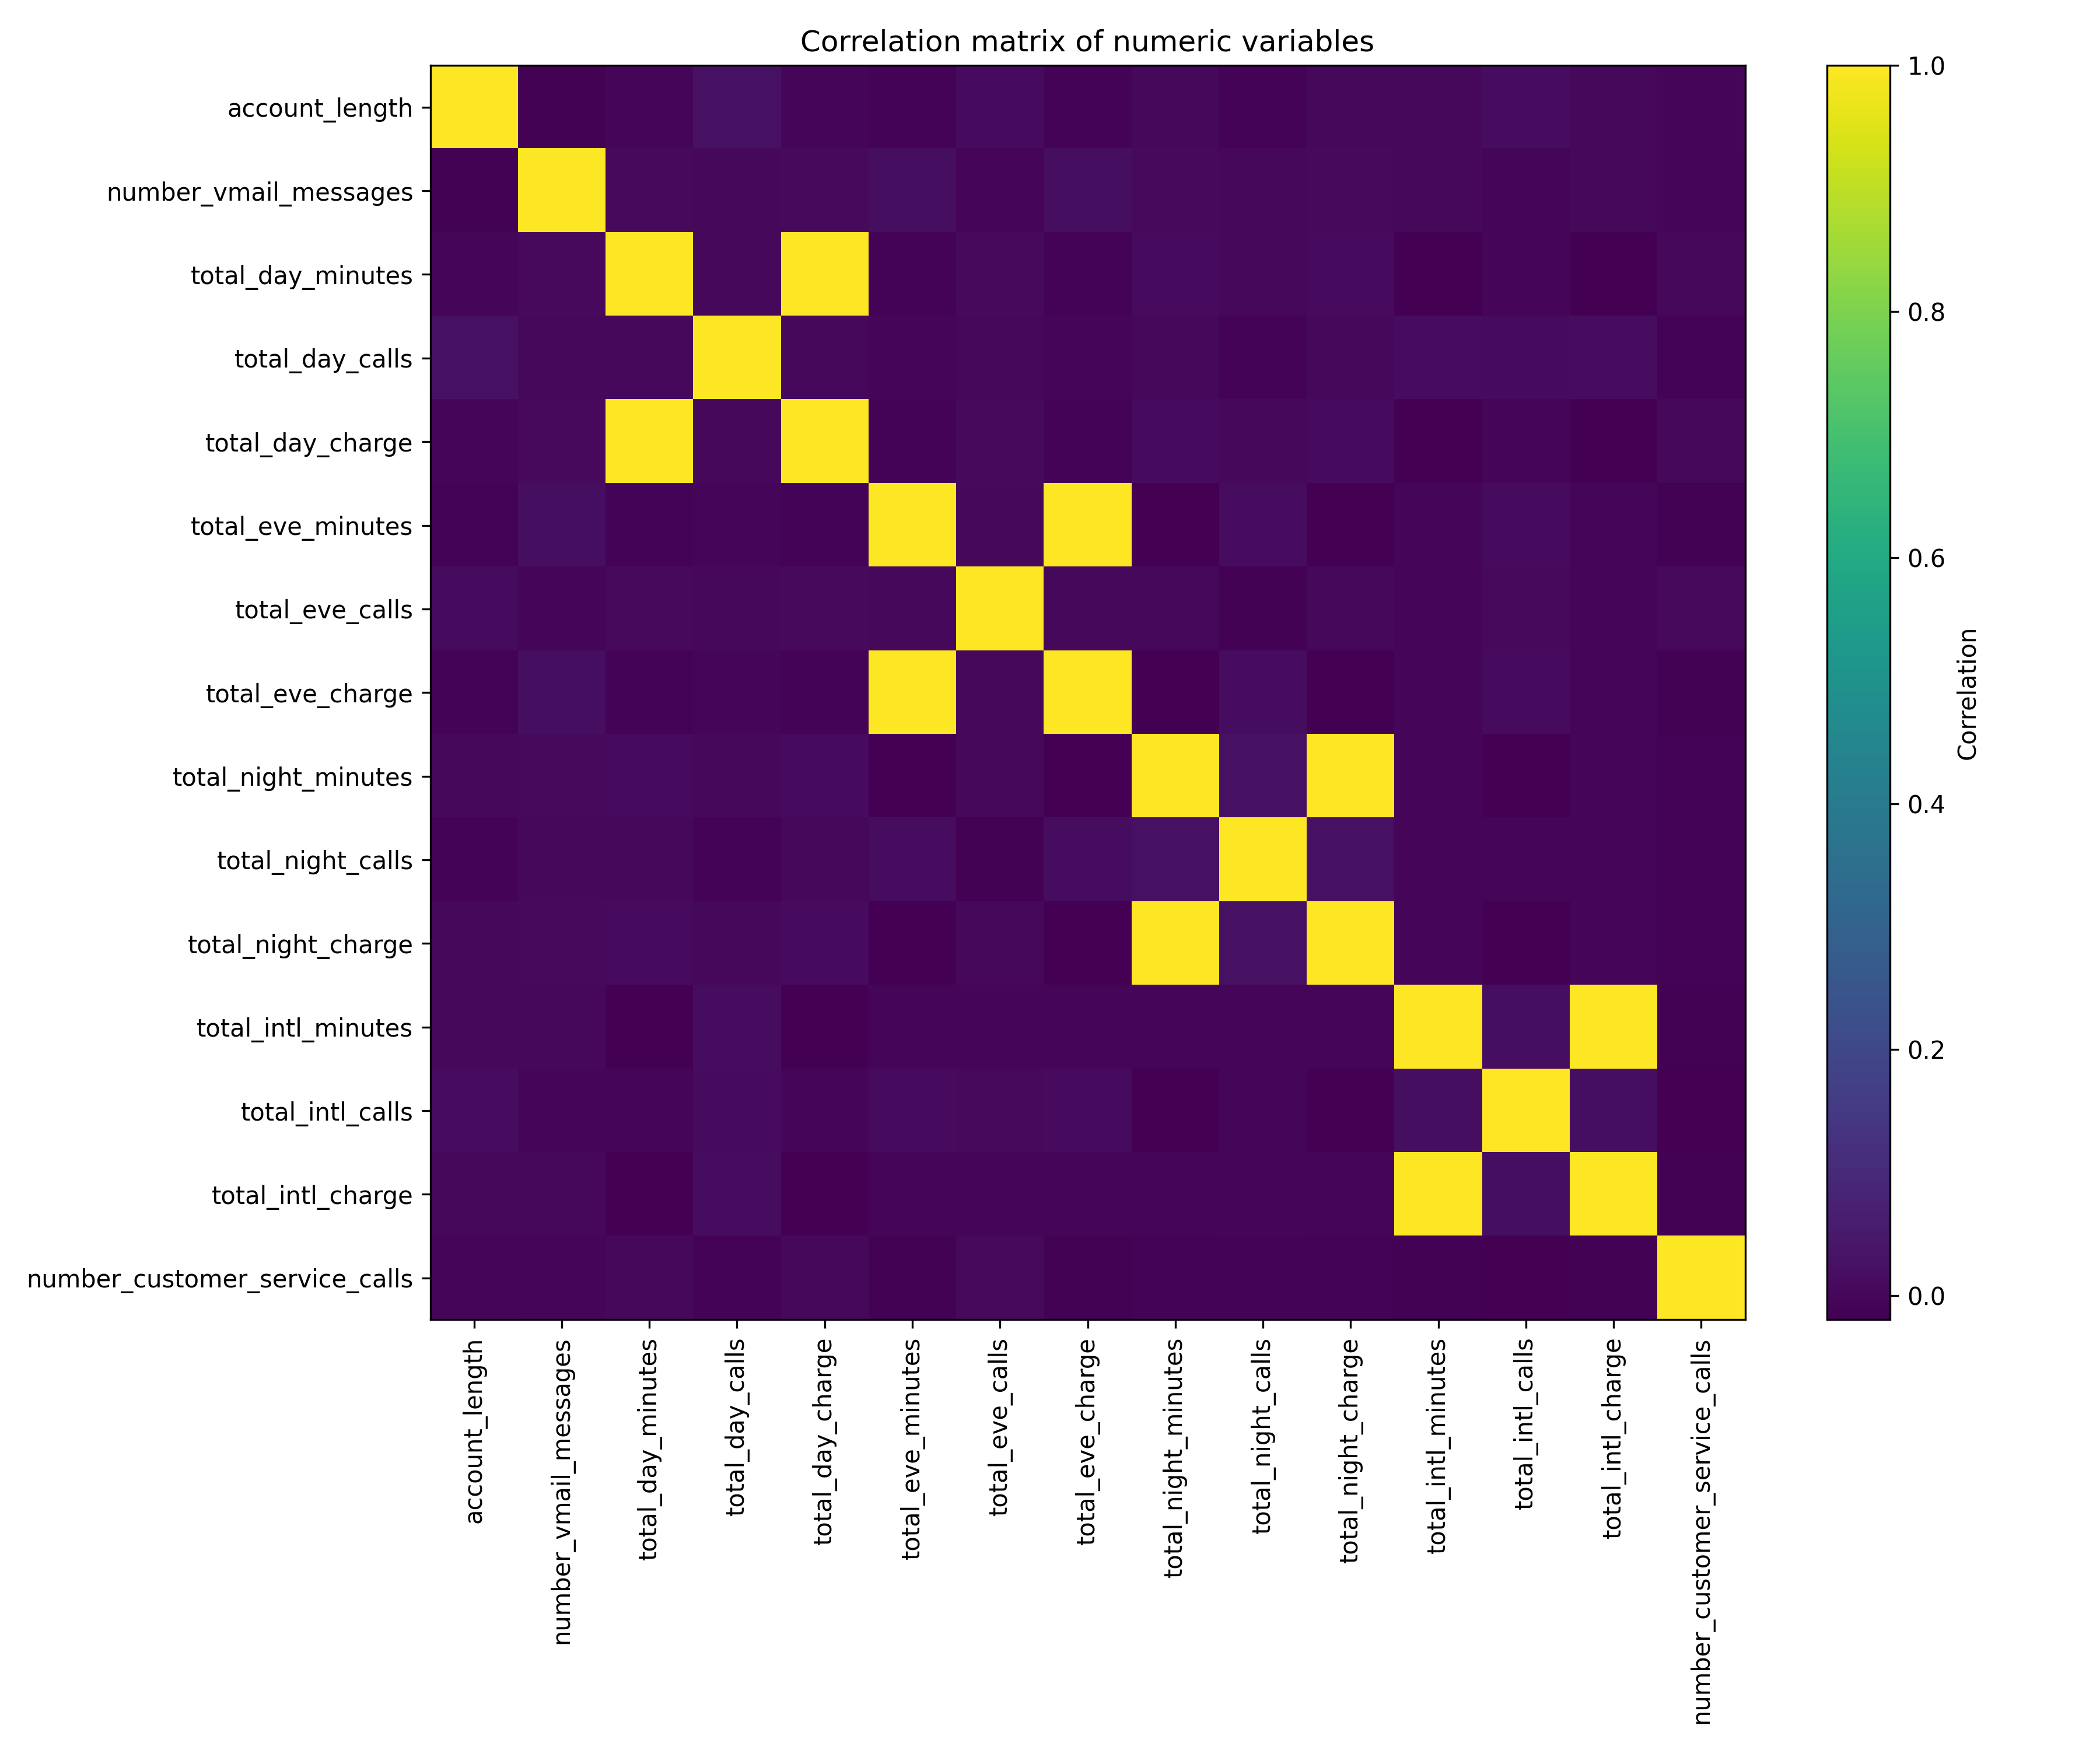
\includegraphics[width=0.95\textwidth]{outputs/correlation_heatmap.png}
    \caption{Ma trận tương quan giữa các biến số.}
    \label{fig:corr_heatmap}
\end{figure}

% ============================================================
\section{Xây dựng mô hình Random Forest}
% ============================================================

\subsection{Mô hình dự đoán}

Mô hình được sử dụng là Random Forest Classifier. Random Forest là thuật toán học máy dựa trên tập hợp nhiều cây quyết định. Mỗi cây được huấn luyện trên một mẫu bootstrap của dữ liệu và tại mỗi nút phân chia, chỉ một tập con ngẫu nhiên các biến được xét. Cách xây dựng này giúp giảm phương sai so với một cây quyết định đơn lẻ và thường cho hiệu năng dự đoán tốt trên dữ liệu dạng bảng.

Trong bài làm, siêu tham số chính được thay đổi là:
\[
\texttt{max\_depth}.
\]
Các siêu tham số khác của Random Forest được giữ ở giá trị mặc định của thư viện \texttt{scikit-learn}. Random seed được đặt bằng 1234 trong tất cả các thí nghiệm nhằm đảm bảo khả năng tái lập kết quả.

\subsection{Tiền xử lý biến đầu vào}

Các biến đầu vào được chia thành hai nhóm:
\begin{itemize}
    \item Biến phân loại: được mã hóa bằng \texttt{OneHotEncoder}.
    \item Biến số: được giữ nguyên.
\end{itemize}

Quá trình tiền xử lý và mô hình Random Forest được đóng gói trong một \texttt{Pipeline}. Việc dùng \texttt{Pipeline} giúp đảm bảo rằng quá trình mã hóa biến phân loại chỉ được học trên tập huấn luyện trong từng fold, tránh rò rỉ thông tin từ tập kiểm tra sang tập huấn luyện.

\subsection{Độ đo đánh giá}

Hiệu năng mô hình được đo bằng F1-score với lớp dương là \texttt{yes}. F1-score được định nghĩa bởi:
\[
F1 = \frac{2 \times Precision \times Recall}{Precision + Recall}.
\]
Trong đó:
\[
Precision = \frac{TP}{TP + FP}, \qquad Recall = \frac{TP}{TP + FN}.
\]

Với bài toán dự đoán rời mạng, lớp \texttt{yes} là lớp quan trọng hơn vì doanh nghiệp thường quan tâm đến việc phát hiện khách hàng có nguy cơ rời mạng. Do đó, F1-score của lớp \texttt{yes} là độ đo phù hợp hơn so với accuracy tổng thể.

% ============================================================
\section{Thu thập dữ liệu hiệu năng mô hình}
% ============================================================

\subsection{Chiến lược đánh giá}

Dữ liệu hiệu năng được thu thập bằng repeated stratified k-fold cross-validation. Do dữ liệu rời mạng thường mất cân bằng giữa hai lớp \texttt{yes} và \texttt{no}, cách chia fold có phân tầng được sử dụng để duy trì tỷ lệ lớp trong từng fold.

Mỗi thí nghiệm sử dụng:
\[
\text{repeat} = 10.
\]
Trong mỗi repeat, dữ liệu được chia thành $k$ fold. Mô hình được huấn luyện trên $k-1$ fold và đánh giá trên fold còn lại. F1-score được tính trên từng fold. Sau đó, F1-score được lấy trung bình theo từng repeat để tạo dữ liệu phân tích ở cấp repeat.

Việc lấy trung bình theo repeat là cần thiết vì số fold khác nhau tạo ra số quan sát fold-level khác nhau. Ví dụ, với 10 repeat:
\[
k=3 \Rightarrow 30 \text{ fold-level scores}, \quad
k=5 \Rightarrow 50 \text{ fold-level scores}, \quad
k=10 \Rightarrow 100 \text{ fold-level scores}.
\]
Nếu phân tích trực tiếp các fold-level scores, nhóm $k=10$ sẽ có nhiều quan sát hơn chỉ vì có nhiều fold hơn, không phải vì có nhiều lần lặp thí nghiệm hơn. Do đó, mỗi repeat được xem là một đơn vị quan sát độc lập trong phân tích thí nghiệm.

\subsection{Dữ liệu kết quả}

Hai file kết quả chính được tạo ra:
\begin{itemize}
    \item \texttt{crd\_results.csv}: kết quả thí nghiệm CRD, gồm 30 quan sát, tương ứng với 3 mức $k$ và 10 repeat cho mỗi mức.
    \item \texttt{crfd\_results.csv}: kết quả thí nghiệm CRFD, gồm 90 quan sát, tương ứng với 3 mức $k$, 3 mức \texttt{max\_depth} và 10 repeat cho mỗi tổ hợp.
\end{itemize}

Ngoài ra, các file fold-level cũng được lưu lại để kiểm tra chi tiết, nhưng không được dùng làm dữ liệu chính cho phân tích thống kê.

% ============================================================
\section{Thí nghiệm CRD}
% ============================================================

\subsection{Thiết kế thí nghiệm}

Thí nghiệm CRD xem xét ảnh hưởng của một yếu tố duy nhất là số fold $k$ trong repeated stratified k-fold. Các mức của yếu tố là:
\[
k \in \{3, 5, 10\}.
\]
Trong thí nghiệm này, \texttt{max\_depth} được giữ cố định ở trạng thái không giới hạn:
\[
\texttt{max\_depth} = \texttt{None}.
\]
Biến đáp ứng là F1-score của lớp \texttt{yes}.

Mô hình phân tích được viết dưới dạng:
\[
F1_{ij} = \mu + \alpha_i + \varepsilon_{ij},
\]
trong đó $\mu$ là trung bình chung, $\alpha_i$ là ảnh hưởng của mức $k_i$, và $\varepsilon_{ij}$ là sai số ngẫu nhiên.

\subsection{Bảng trung bình và khoảng tin cậy}

Bảng \ref{tab:crd_summary} trình bày F1 trung bình và khoảng tin cậy 95\% cho từng mức $k$.

\begin{table}[H]
    \centering
    \caption{Kết quả trung bình F1 và khoảng tin cậy 95\% trong thí nghiệm CRD.}
    \label{tab:crd_summary}
    \begin{tabular}{ccccc}
        \toprule
        $k$ & $n$ & Trung bình F1 & Độ lệch chuẩn & Khoảng tin cậy 95\% \\
        \midrule
        3  & 10 & 0.790 & 0.00742 & [0.785, 0.795] \\
        5  & 10 & 0.798 & 0.00607 & [0.793, 0.802] \\
        10 & 10 & 0.807 & 0.00605 & [0.803, 0.812] \\
        \bottomrule
    \end{tabular}
\end{table}

Kết quả cho thấy F1-score trung bình tăng dần khi số fold tăng từ 3 lên 10. Cụ thể, $k=3$ đạt F1 trung bình khoảng 0.790, $k=5$ đạt khoảng 0.798 và $k=10$ đạt khoảng 0.807.

\begin{figure}[H]
    \centering
    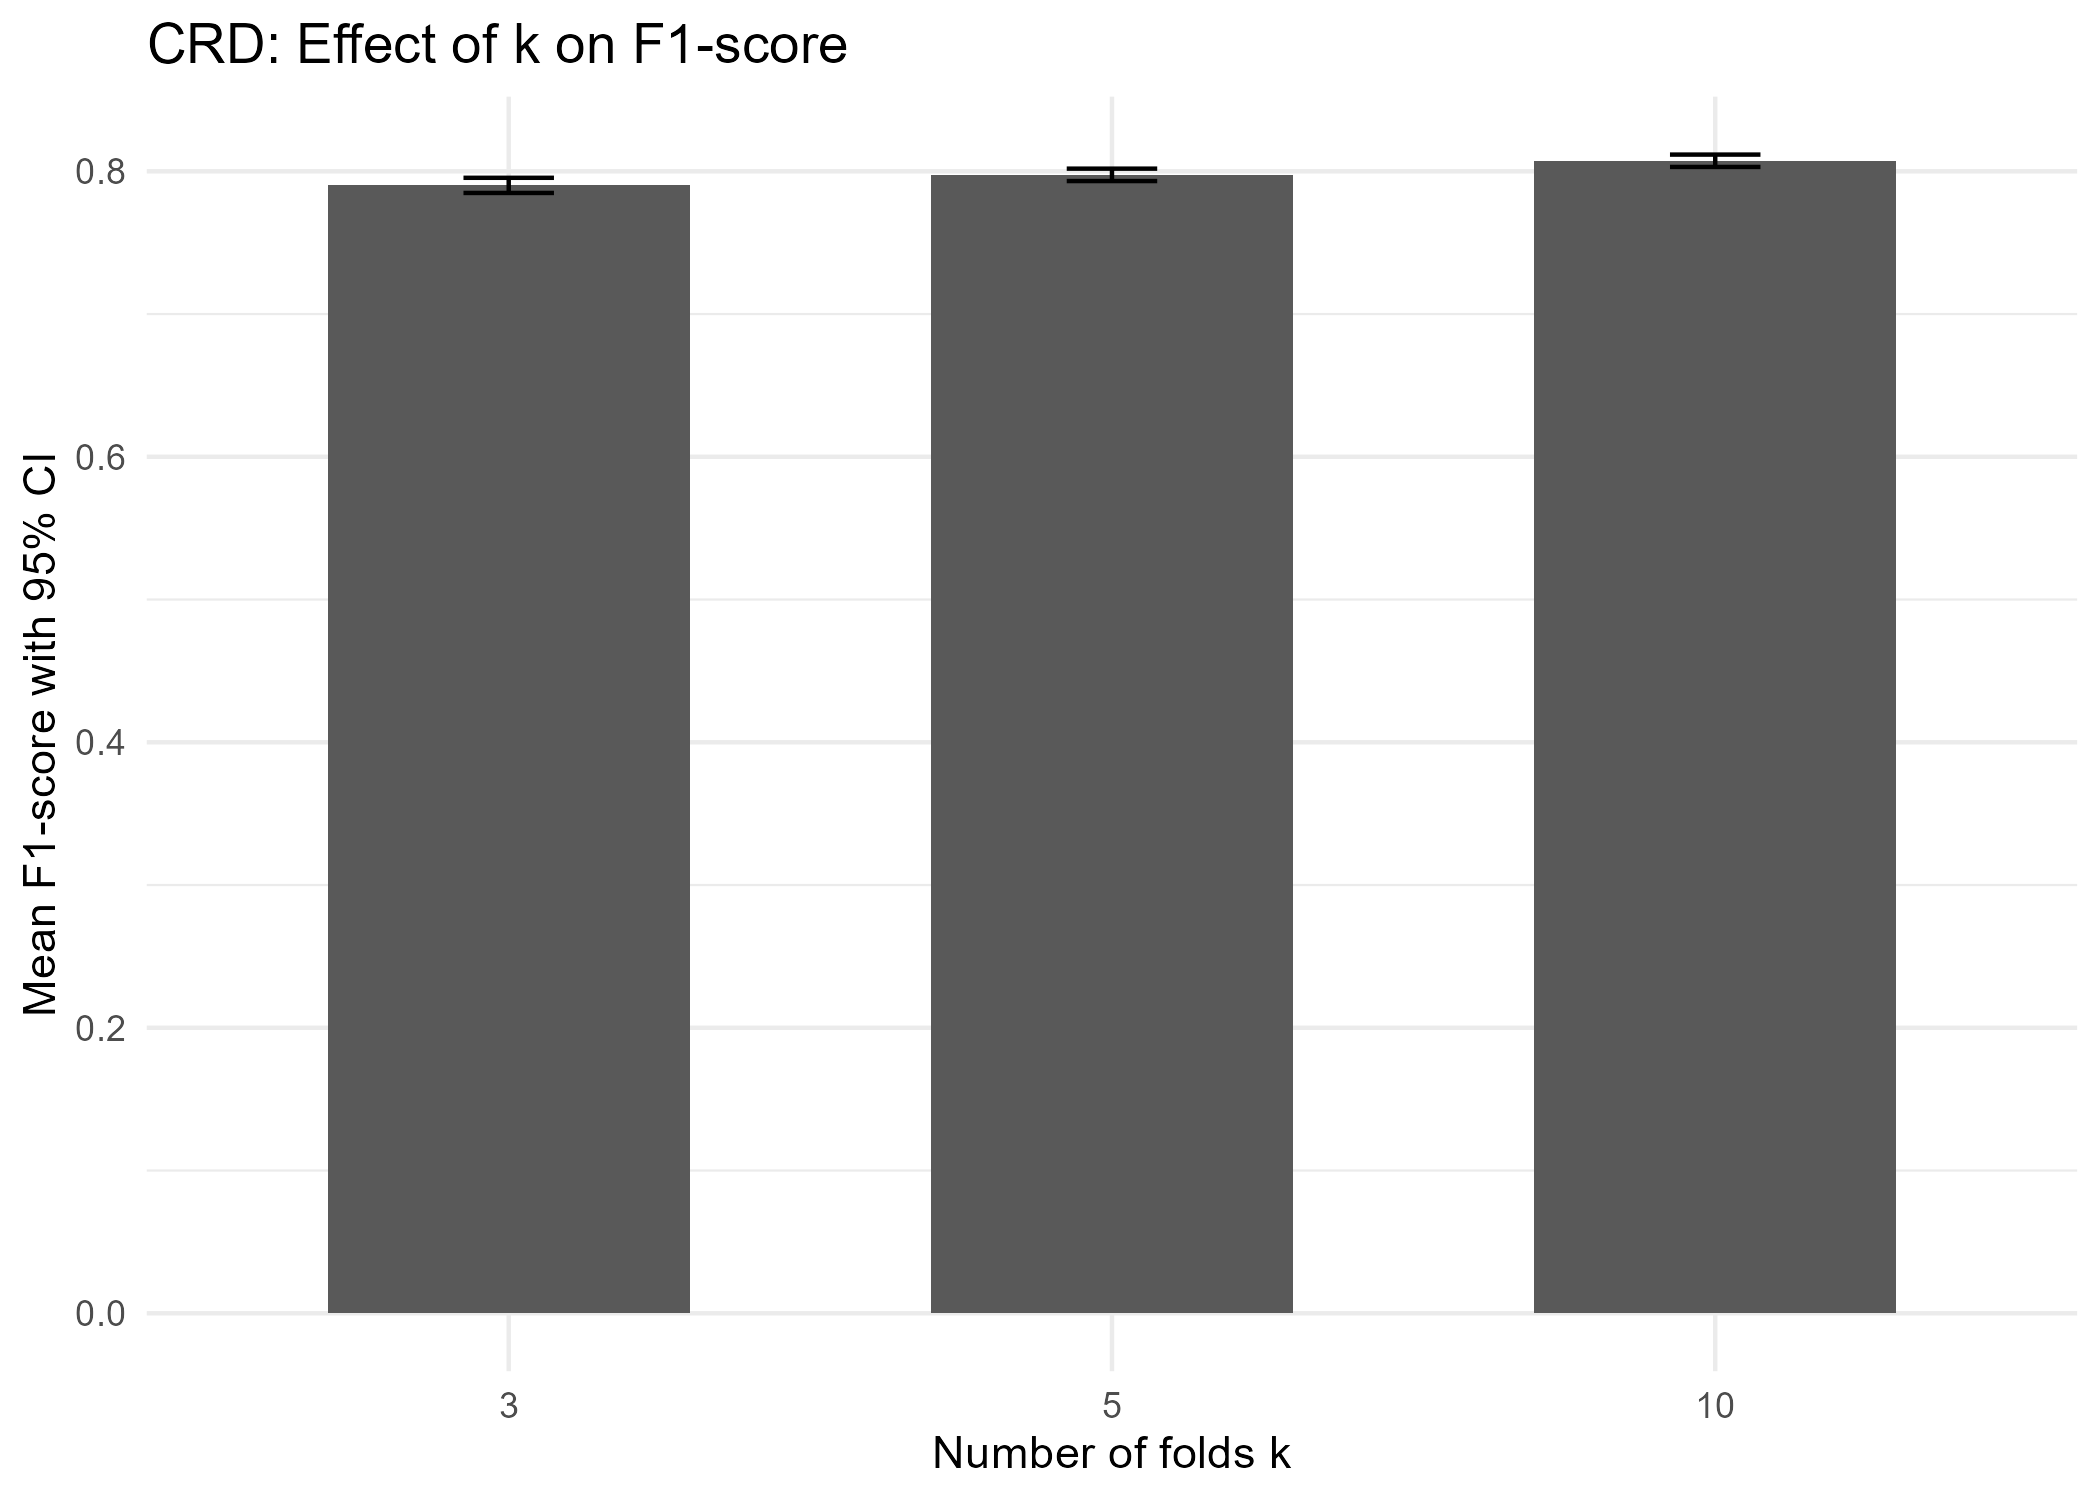
\includegraphics[width=0.78\textwidth]{outputs/r_crd_mean_ci_plot.png}
    \caption{Trung bình F1 và khoảng tin cậy 95\% theo số fold $k$ trong thí nghiệm CRD.}
    \label{fig:crd_mean_ci}
\end{figure}

Hình \ref{fig:crd_mean_ci} cho thấy xu hướng tăng rõ ràng của F1-score khi $k$ tăng. Khoảng tin cậy của $k=10$ nằm cao hơn đáng kể so với $k=3$, gợi ý rằng sử dụng nhiều fold hơn giúp ước lượng hiệu năng mô hình tốt hơn trong thí nghiệm này.

\subsection{Phân bố F1 theo từng mức k}

Hình \ref{fig:crd_boxplot} biểu diễn phân bố F1-score theo từng mức $k$. Các điểm trên hình là các giá trị F1 của từng repeat. Đường ngang trong mỗi hộp là trung vị, hộp biểu diễn khoảng tứ phân vị và râu thể hiện mức dao động chính của dữ liệu.

\begin{figure}[H]
    \centering
    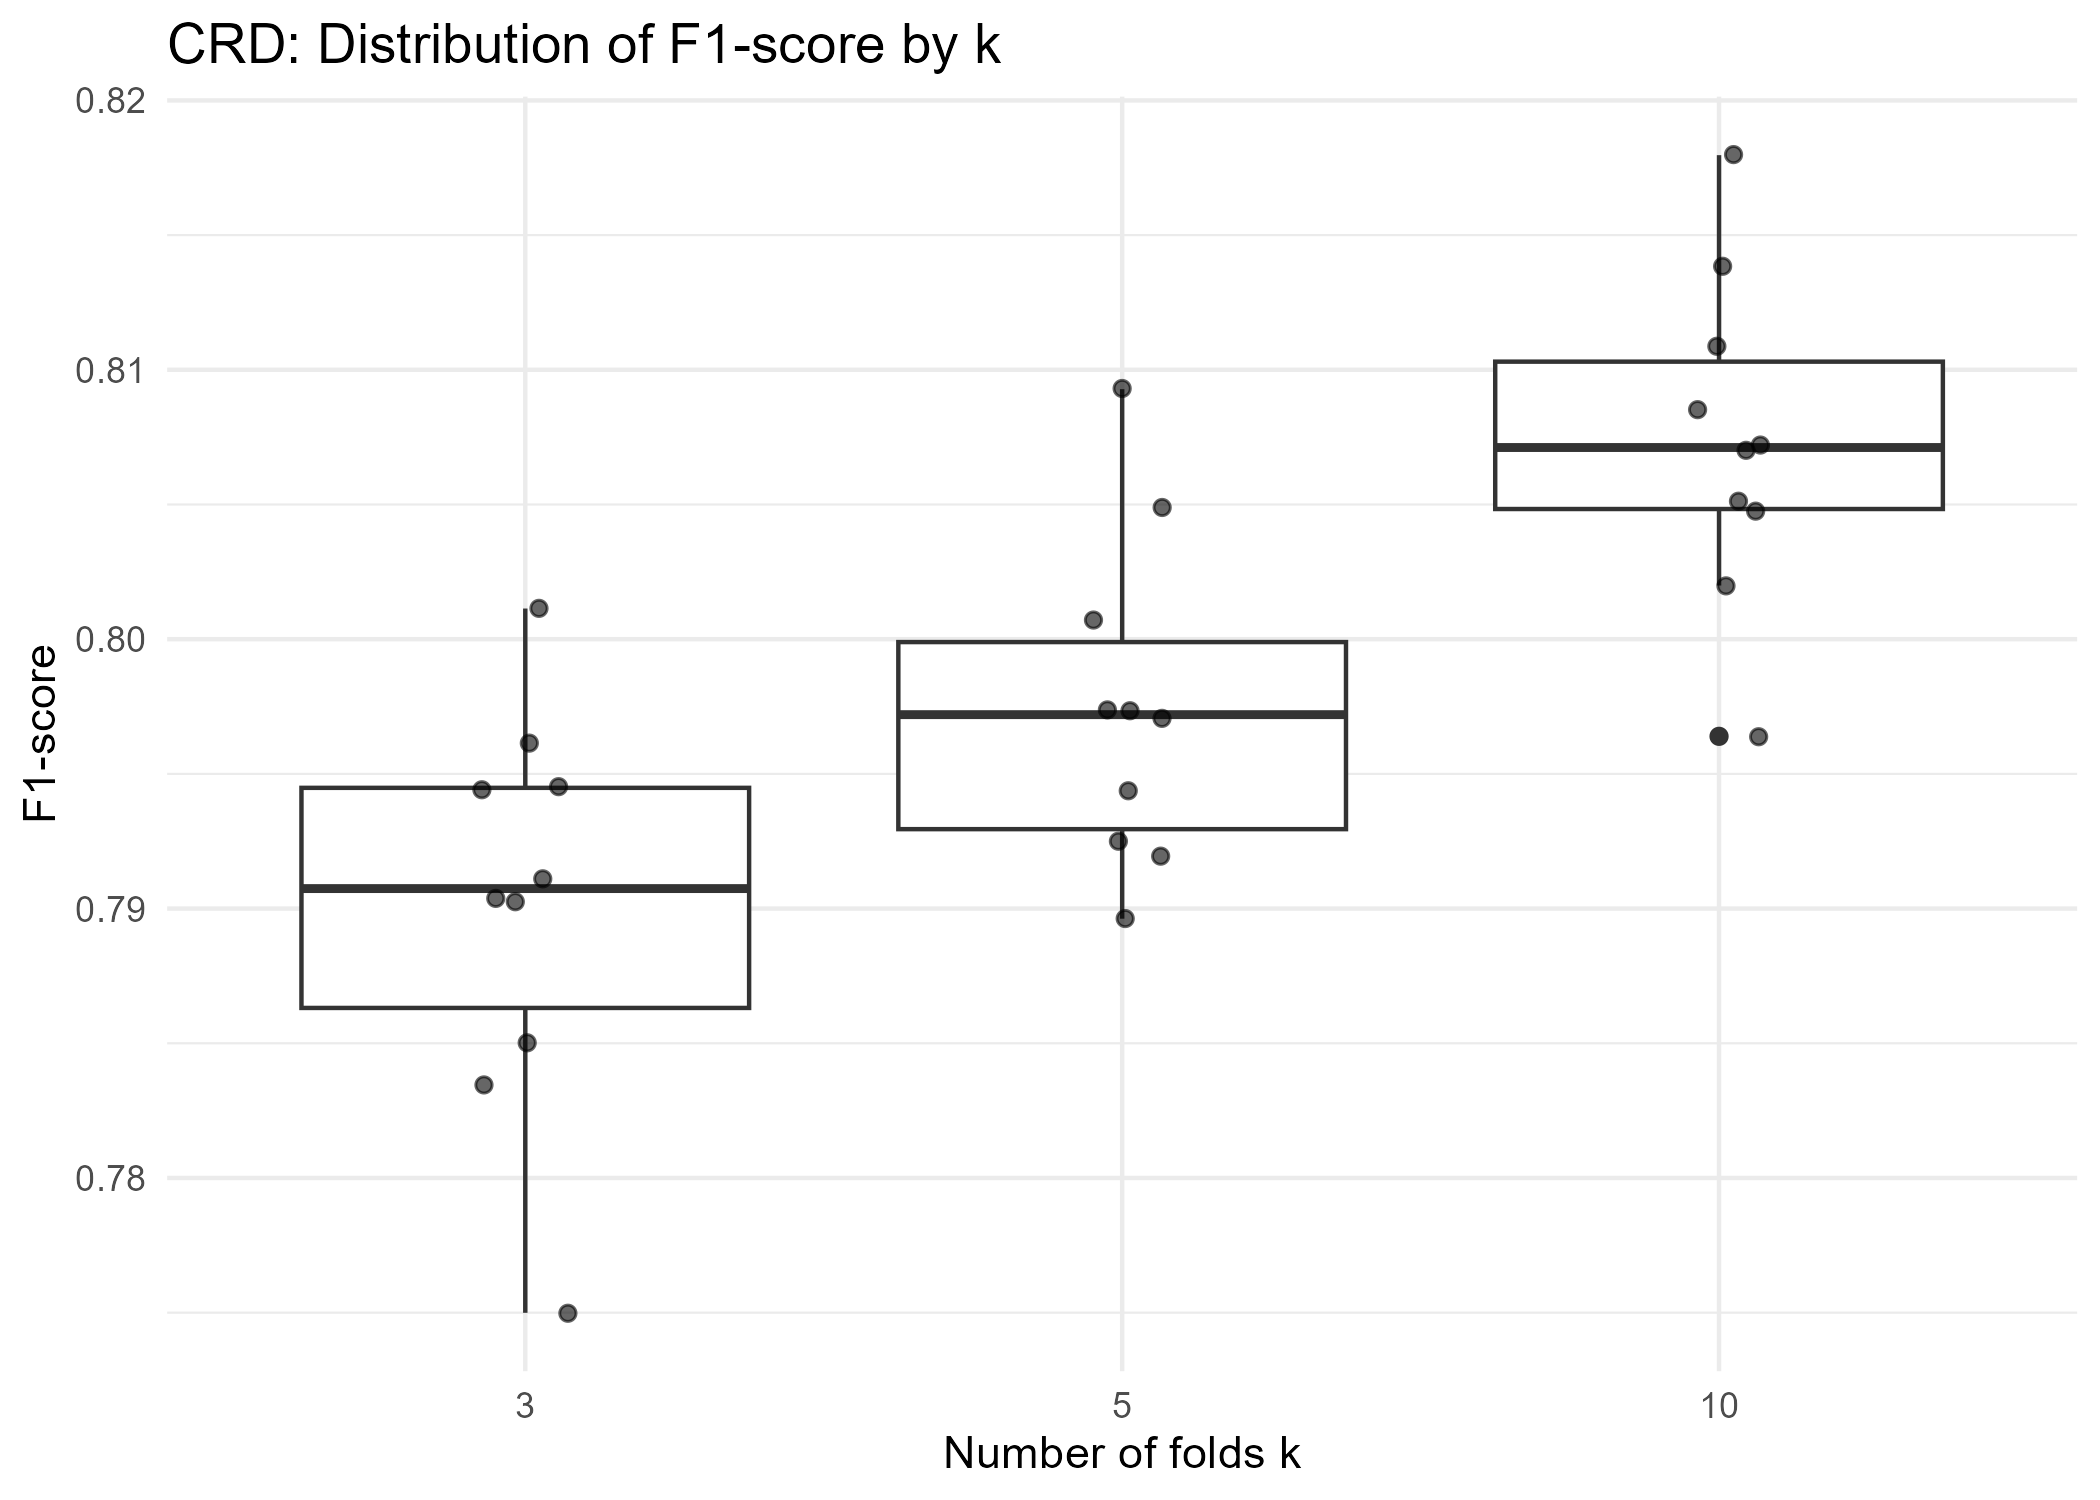
\includegraphics[width=0.85\textwidth]{outputs/r_crd_boxplot.png}
    \caption{Boxplot phân bố F1-score theo số fold $k$ trong thí nghiệm CRD.}
    \label{fig:crd_boxplot}
\end{figure}

Từ boxplot có thể thấy nhóm $k=10$ có mức F1 cao hơn hai nhóm còn lại. Nhóm $k=3$ có F1 thấp nhất và có một vài giá trị thấp hơn đáng kể, cho thấy việc dùng ít fold hơn có thể làm ước lượng hiệu năng kém ổn định hơn.

\subsection{Kiểm định Levene về phương sai}

Trước khi phân tích ảnh hưởng của $k$, kiểm định Levene được sử dụng để so sánh phương sai F1 giữa ba nhóm. Giả thuyết kiểm định là:
\[
H_0: \sigma_3^2 = \sigma_5^2 = \sigma_{10}^2.
\]

Kết quả kiểm định Levene:
\[
F = 0.1663, \qquad p = 0.8476.
\]

Vì $p = 0.8476 > 0.05$, không có bằng chứng để bác bỏ giả thuyết không. Do đó, có thể xem phương sai F1 giữa các mức $k$ là tương đương. Điều này hỗ trợ việc sử dụng mô hình tuyến tính và ANOVA để so sánh trung bình giữa các nhóm.

\subsection{Phân tích ANOVA bằng mô hình tuyến tính}

Mô hình tuyến tính được sử dụng:
\[
\texttt{lm}(F1 \sim k).
\]

Kết quả ANOVA cho thấy:
\[
F = 17.445, \qquad p = 1.369 \times 10^{-5}.
\]

Vì $p < 0.05$, yếu tố $k$ có ảnh hưởng có ý nghĩa thống kê đến F1-score. Nói cách khác, hiệu năng mô hình Random Forest thay đổi đáng kể khi thay đổi số fold $k$ trong repeated stratified k-fold.

Trong mô hình hồi quy tuyến tính, mức tham chiếu là $k=3$. Hệ số của $k=5$ là 0.007373 với $p = 0.018$, cho thấy F1 trung bình của $k=5$ cao hơn $k=3$ khoảng 0.00737 và khác biệt có ý nghĩa thống kê ở mức 5\%. Hệ số của $k=10$ là 0.017236 với $p = 2.86 \times 10^{-6}$, cho thấy $k=10$ cao hơn $k=3$ khoảng 0.01724 và khác biệt rất có ý nghĩa thống kê.

\subsection{So sánh hậu nghiệm TukeyHSD}

Sau khi ANOVA cho thấy có khác biệt giữa các mức $k$, kiểm định TukeyHSD được dùng để so sánh từng cặp nhóm. Kết quả được trình bày trong Bảng \ref{tab:crd_tukey}.

\begin{table}[H]
    \centering
    \caption{Kết quả TukeyHSD cho thí nghiệm CRD.}
    \label{tab:crd_tukey}
    \begin{tabular}{ccccc}
        \toprule
        So sánh & Chênh lệch & Cận dưới & Cận trên & p-value hiệu chỉnh \\
        \midrule
        5 - 3   & 0.00737 & 0.00011 & 0.01463 & 0.04602 \\
        10 - 3  & 0.01724 & 0.00998 & 0.02450 & 0.0000083 \\
        10 - 5  & 0.00986 & 0.00260 & 0.01712 & 0.00626 \\
        \bottomrule
    \end{tabular}
\end{table}

Kết quả TukeyHSD cho thấy cả ba cặp so sánh đều có khác biệt có ý nghĩa thống kê ở mức 5\%. Trong đó, $k=10$ cho F1 cao hơn đáng kể so với cả $k=3$ và $k=5$. Đồng thời, $k=5$ cũng cao hơn $k=3$. Như vậy, trong thí nghiệm CRD, lựa chọn $k=10$ cho kết quả tốt nhất.

\begin{figure}[H]
    \centering
    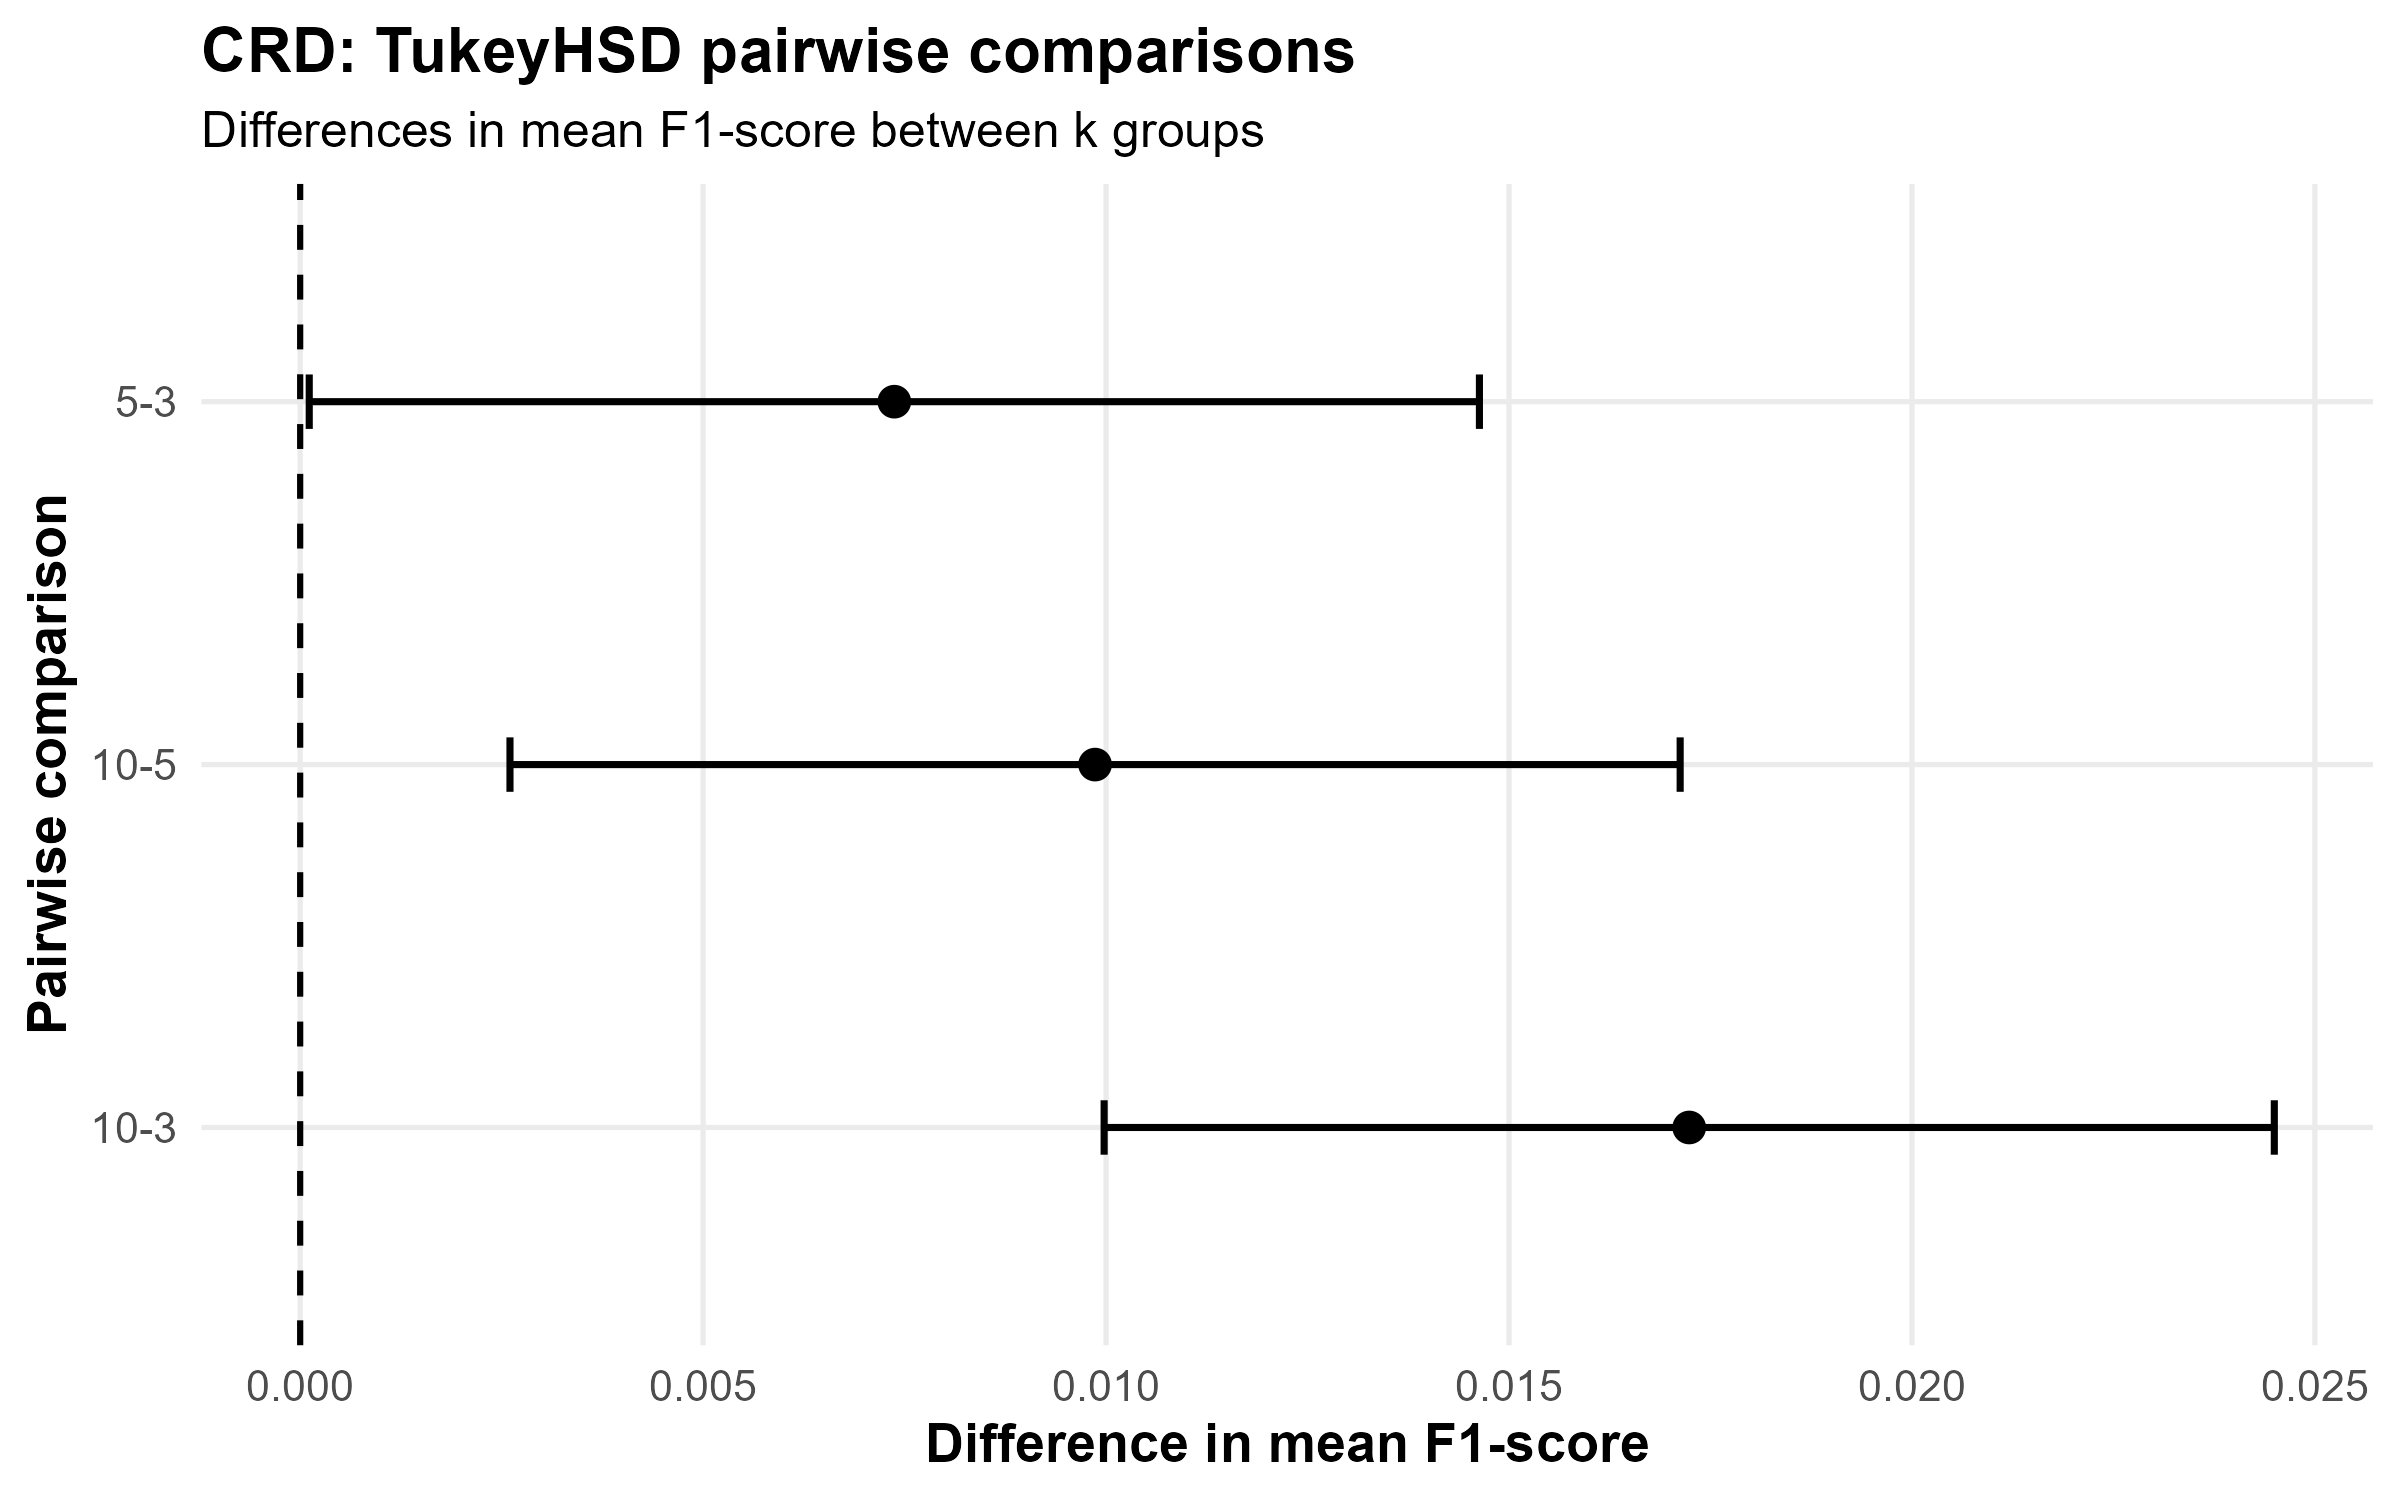
\includegraphics[width=0.85\textwidth]{outputs/r_crd_tukey_plot.png}
    \caption{Đồ thị TukeyHSD so sánh các mức $k$ trong thí nghiệm CRD.}
    \label{fig:crd_tukey}
\end{figure}

\subsection{Kiểm tra giả định phần dư}

Kiểm định Shapiro-Wilk được dùng để kiểm tra giả định phân phối chuẩn của phần dư trong mô hình CRD. Kết quả:
\[
W = 0.98056, \qquad p = 0.8402.
\]
Vì $p > 0.05$, không có bằng chứng cho thấy phần dư lệch khỏi phân phối chuẩn. Điều này cho thấy giả định phân phối chuẩn của phần dư là phù hợp đối với mô hình CRD.

\begin{figure}[H]
    \centering
    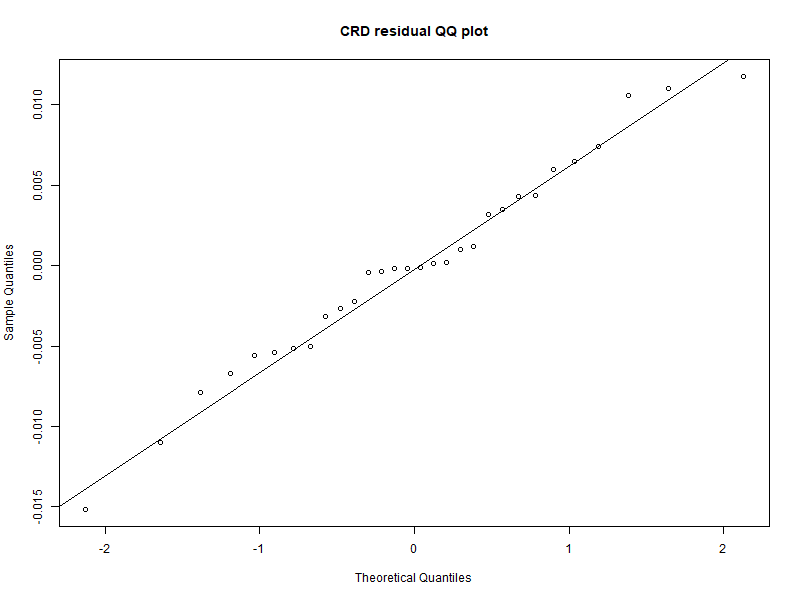
\includegraphics[width=0.72\textwidth]{outputs/r_crd_qqplot.png}
    \caption{QQ plot phần dư của mô hình CRD.}
    \label{fig:crd_qqplot}
\end{figure}

% ============================================================
\section{Thí nghiệm CRFD}
% ============================================================

\subsection{Thiết kế thí nghiệm}

Thí nghiệm CRFD xem xét đồng thời hai yếu tố:
\[
k \in \{3, 5, 10\},
\]
và:
\[
\texttt{max\_depth} \in \{3, 5, \texttt{None}\}.
\]

Tổng cộng có:
\[
3 \times 3 = 9
\]
tổ hợp nghiệm thức. Mỗi tổ hợp được lặp lại 10 lần, tương ứng với 10 repeat. Do đó, dữ liệu phân tích CRFD có 90 quan sát.

Mô hình phân tích có dạng:
\[
F1_{ijk} = \mu + \alpha_i + \beta_j + (\alpha\beta)_{ij} + \varepsilon_{ijk},
\]
trong đó $\alpha_i$ là ảnh hưởng của yếu tố $k$, $\beta_j$ là ảnh hưởng của yếu tố \texttt{max\_depth}, và $(\alpha\beta)_{ij}$ là ảnh hưởng tương tác giữa hai yếu tố.

\subsection{Bảng trung bình và khoảng tin cậy}

Bảng \ref{tab:crfd_summary} trình bày F1 trung bình và khoảng tin cậy 95\% cho từng tổ hợp $k$ và \texttt{max\_depth}.

\begin{table}[H]
    \centering
    \caption{Kết quả trung bình F1 và khoảng tin cậy 95\% trong thí nghiệm CRFD.}
    \label{tab:crfd_summary}
    \begin{tabular}{cccccc}
        \toprule
        $k$ & \texttt{max\_depth} & $n$ & Trung bình F1 & Độ lệch chuẩn & Khoảng tin cậy 95\% \\
        \midrule
        3  & 3    & 10 & 0.0571 & 0.00542 & [0.0532, 0.0609] \\
        3  & 5    & 10 & 0.575  & 0.0141  & [0.565, 0.585] \\
        3  & None & 10 & 0.790  & 0.00742 & [0.785, 0.795] \\
        5  & 3    & 10 & 0.0608 & 0.00587 & [0.0566, 0.0650] \\
        5  & 5    & 10 & 0.595  & 0.0134  & [0.585, 0.604] \\
        5  & None & 10 & 0.798  & 0.00607 & [0.793, 0.802] \\
        10 & 3    & 10 & 0.0545 & 0.00410 & [0.0515, 0.0574] \\
        10 & 5    & 10 & 0.594  & 0.00956 & [0.587, 0.601] \\
        10 & None & 10 & 0.807  & 0.00605 & [0.803, 0.812] \\
        \bottomrule
    \end{tabular}
\end{table}

Kết quả cho thấy \texttt{max\_depth} có ảnh hưởng rất lớn đến F1-score. Khi \texttt{max\_depth = 3}, F1 chỉ khoảng 0.05--0.06, cho thấy mô hình bị giới hạn độ sâu quá mạnh và không học được cấu trúc phân biệt lớp \texttt{yes}. Khi \texttt{max\_depth = 5}, F1 tăng lên khoảng 0.575--0.595. Khi không giới hạn độ sâu, F1 đạt mức cao nhất, khoảng 0.790--0.807.

\subsection{Phân tích mô hình hiệu ứng chính}

Trước hết, mô hình chỉ gồm hiệu ứng chính được xét:
\[
\texttt{lm}(F1 \sim k + \texttt{max\_depth}).
\]

Kết quả ANOVA cho mô hình hiệu ứng chính cho thấy:
\[
p_k = 2.257 \times 10^{-5}, \qquad
p_{\texttt{max\_depth}} < 2.2 \times 10^{-16}.
\]

Như vậy, cả hai yếu tố $k$ và \texttt{max\_depth} đều có ảnh hưởng có ý nghĩa thống kê đến F1-score. Tuy nhiên, giá trị F rất lớn của \texttt{max\_depth} cho thấy đây là yếu tố chi phối mạnh hơn nhiều so với $k$.

\subsection{Phân tích mô hình có tương tác}

Để kiểm tra xem ảnh hưởng của $k$ có phụ thuộc vào \texttt{max\_depth} hay không, mô hình tương tác được sử dụng:
\[
\texttt{lm}(F1 \sim k * \texttt{max\_depth}).
\]

Kết quả ANOVA của mô hình tương tác được trình bày trong Bảng \ref{tab:crfd_anova}.

\begin{table}[H]
    \centering
    \caption{ANOVA cho mô hình tương tác CRFD.}
    \label{tab:crfd_anova}
    \begin{tabular}{ccccc}
        \toprule
        Nguồn biến thiên & Df & Sum Sq & F value & p-value \\
        \midrule
        $k$ & 2 & 0.002 & 15.079 & $2.71 \times 10^{-6}$ \\
        \texttt{max\_depth} & 2 & 8.746 & 58057.369 & $< 2 \times 10^{-16}$ \\
        $k:\texttt{max\_depth}$ & 4 & 0.002 & 6.088 & 0.000247 \\
        Residuals & 81 & 0.006 & -- & -- \\
        \bottomrule
    \end{tabular}
\end{table}

Kết quả cho thấy:
\begin{itemize}
    \item Yếu tố $k$ có ảnh hưởng có ý nghĩa thống kê đến F1-score.
    \item Yếu tố \texttt{max\_depth} có ảnh hưởng rất mạnh và có ý nghĩa thống kê đến F1-score.
    \item Tương tác giữa $k$ và \texttt{max\_depth} cũng có ý nghĩa thống kê với $p = 0.000247$.
\end{itemize}

Điều này có nghĩa là ảnh hưởng của số fold $k$ đến F1-score không hoàn toàn giống nhau tại các mức \texttt{max\_depth}. Nói cách khác, tác động của $k$ phụ thuộc vào việc cây trong Random Forest bị giới hạn độ sâu ở mức nào.

\subsection{Đồ thị tương tác}

Hình \ref{fig:crfd_interaction} trình bày đồ thị tương tác giữa $k$ và \texttt{max\_depth}.

\begin{figure}[H]
    \centering
    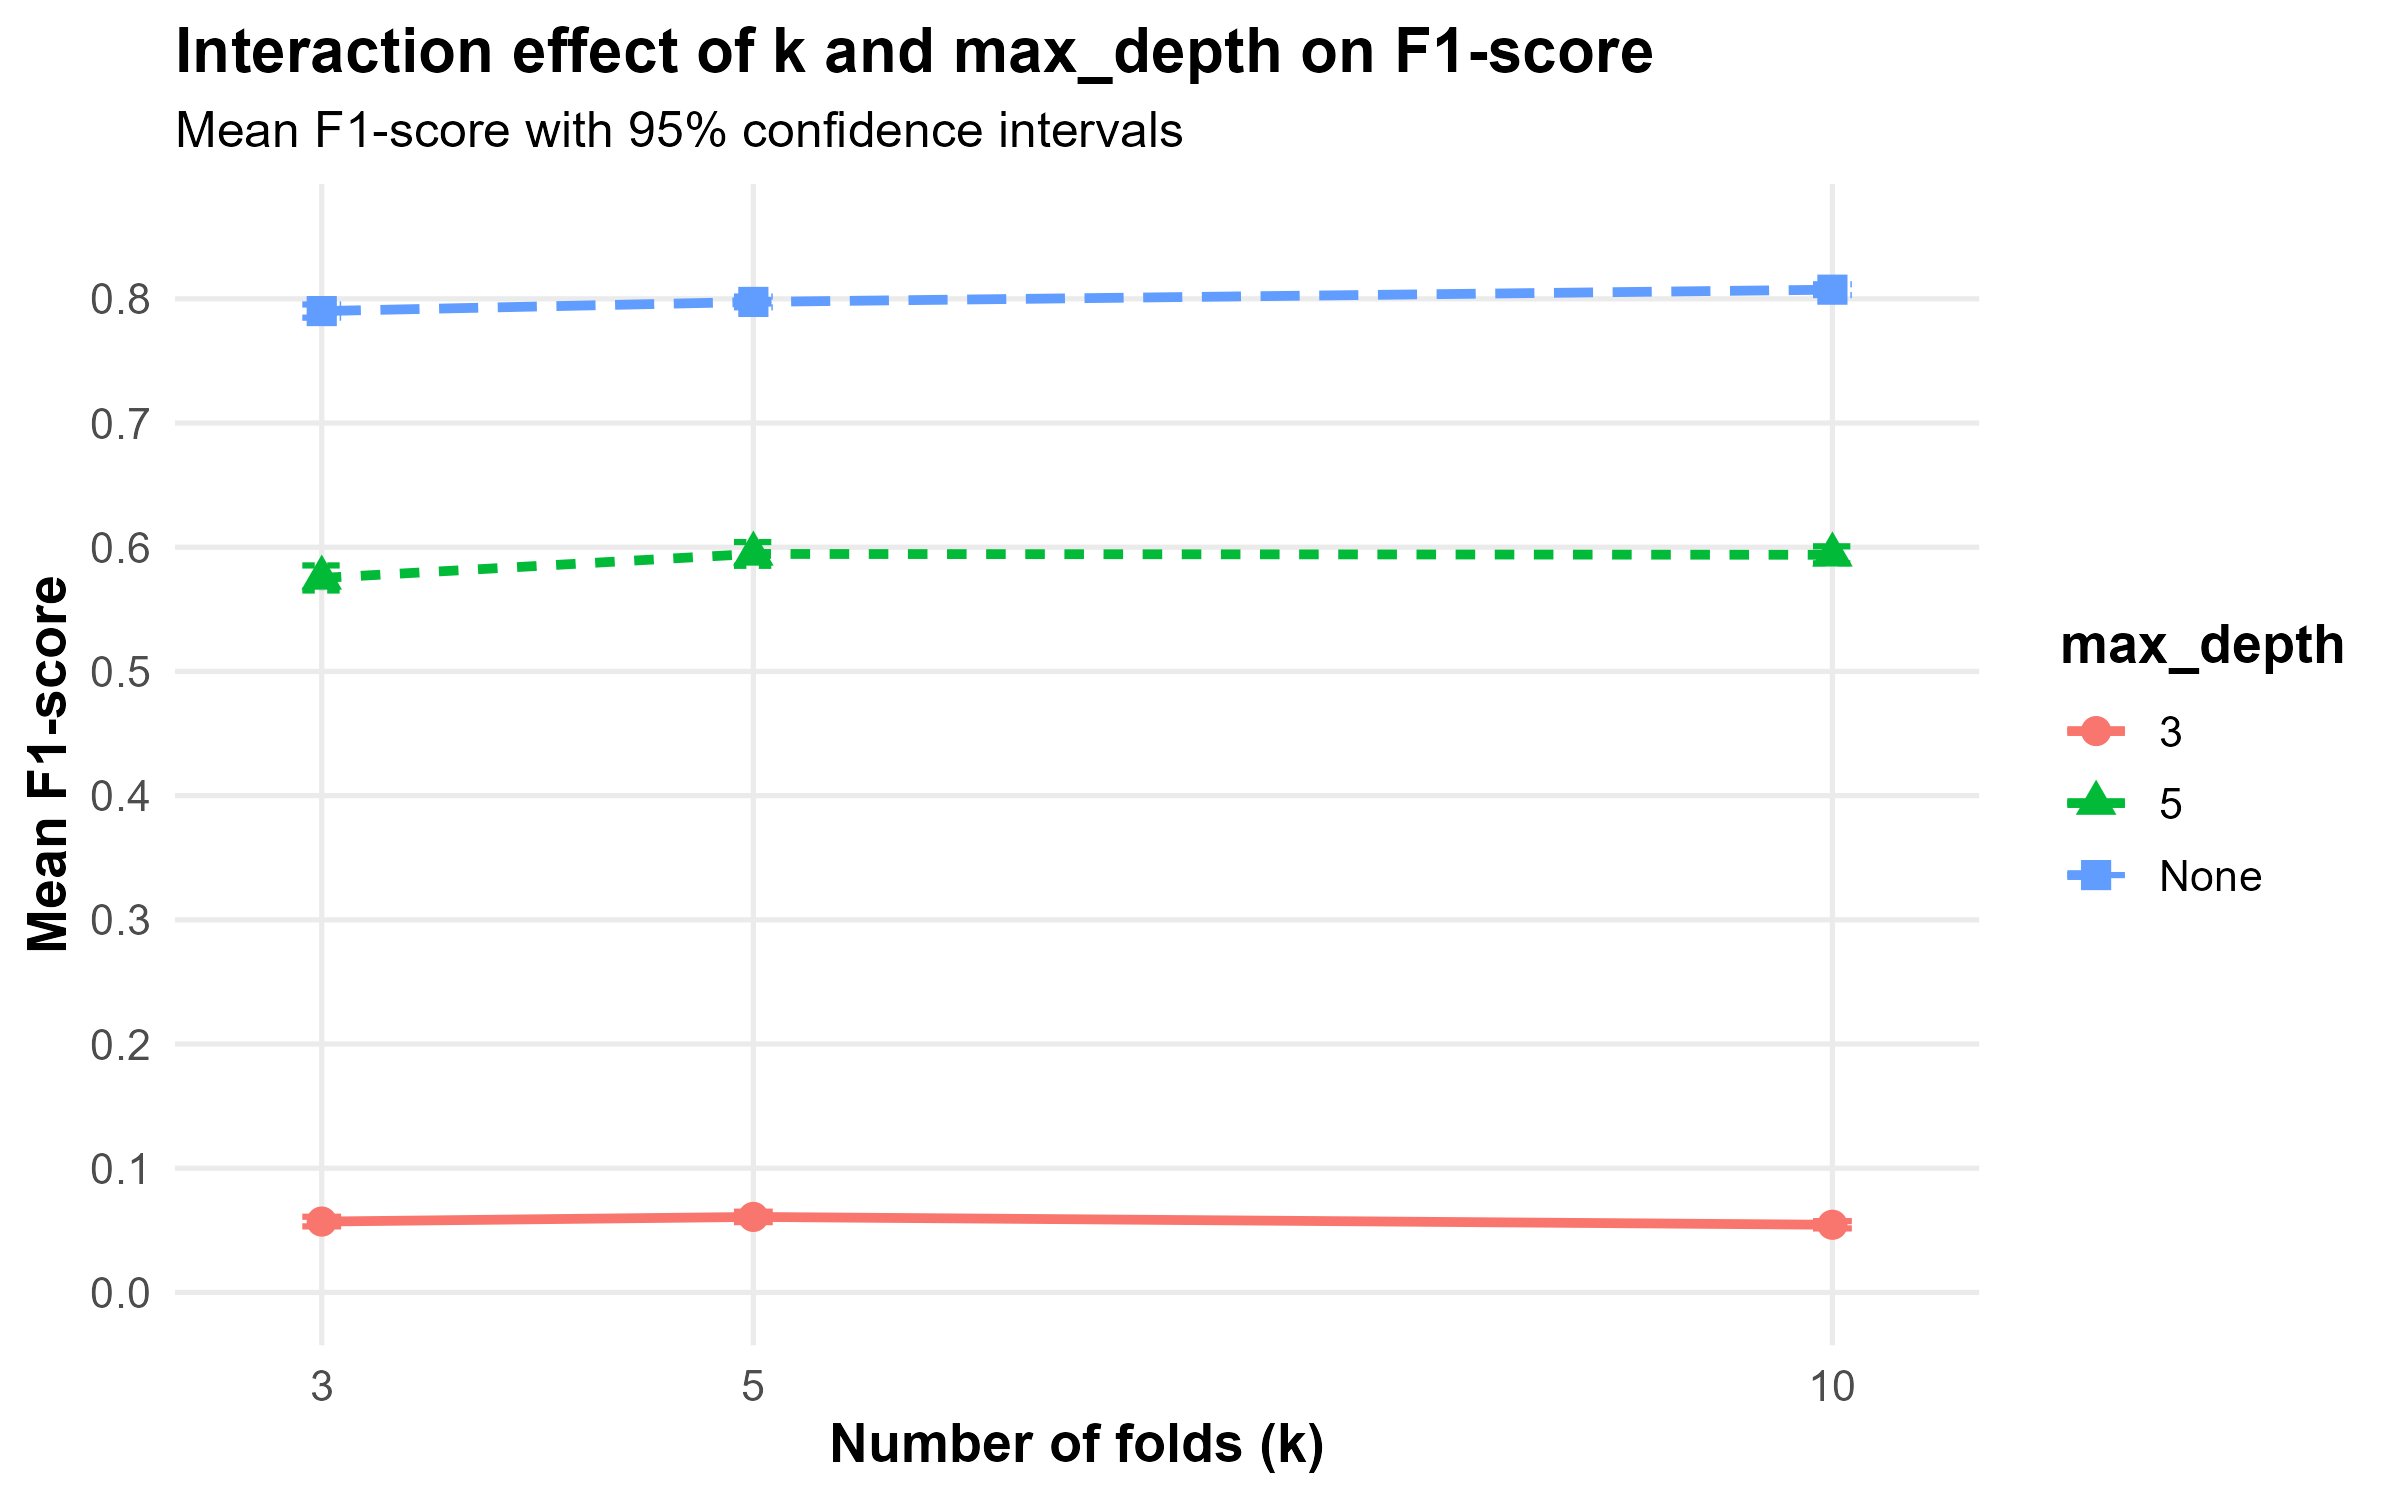
\includegraphics[width=0.88\textwidth]{outputs/r_crfd_interaction_plot.png}
    \caption{Đồ thị tương tác giữa số fold $k$ và \texttt{max\_depth}.}
    \label{fig:crfd_interaction}
\end{figure}

Đồ thị cho thấy ba đường ứng với ba mức \texttt{max\_depth} nằm ở các vùng F1 rất khác nhau. Đường \texttt{max\_depth = None} luôn nằm cao nhất, tiếp theo là \texttt{max\_depth = 5}, còn \texttt{max\_depth = 3} nằm rất thấp. Điều này xác nhận rằng độ sâu cây là yếu tố quan trọng nhất trong thí nghiệm.

Đối với \texttt{max\_depth = None}, F1 tăng khi $k$ tăng từ 3 lên 10. Đối với \texttt{max\_depth = 5}, F1 tăng từ $k=3$ lên $k=5$ và gần như giữ ổn định ở $k=10$. Đối với \texttt{max\_depth = 3}, F1 rất thấp ở cả ba mức $k$, cho thấy mô hình bị underfitting nghiêm trọng. Sự khác nhau về hình dạng các đường là nguyên nhân làm tương tác $k:\texttt{max\_depth}$ có ý nghĩa thống kê.

\subsection{Phân bố F1 theo tổ hợp yếu tố}

Hình \ref{fig:crfd_boxplot} cho thấy phân bố F1 theo \texttt{max\_depth}, chia riêng theo từng mức $k$.

\begin{figure}[H]
    \centering
    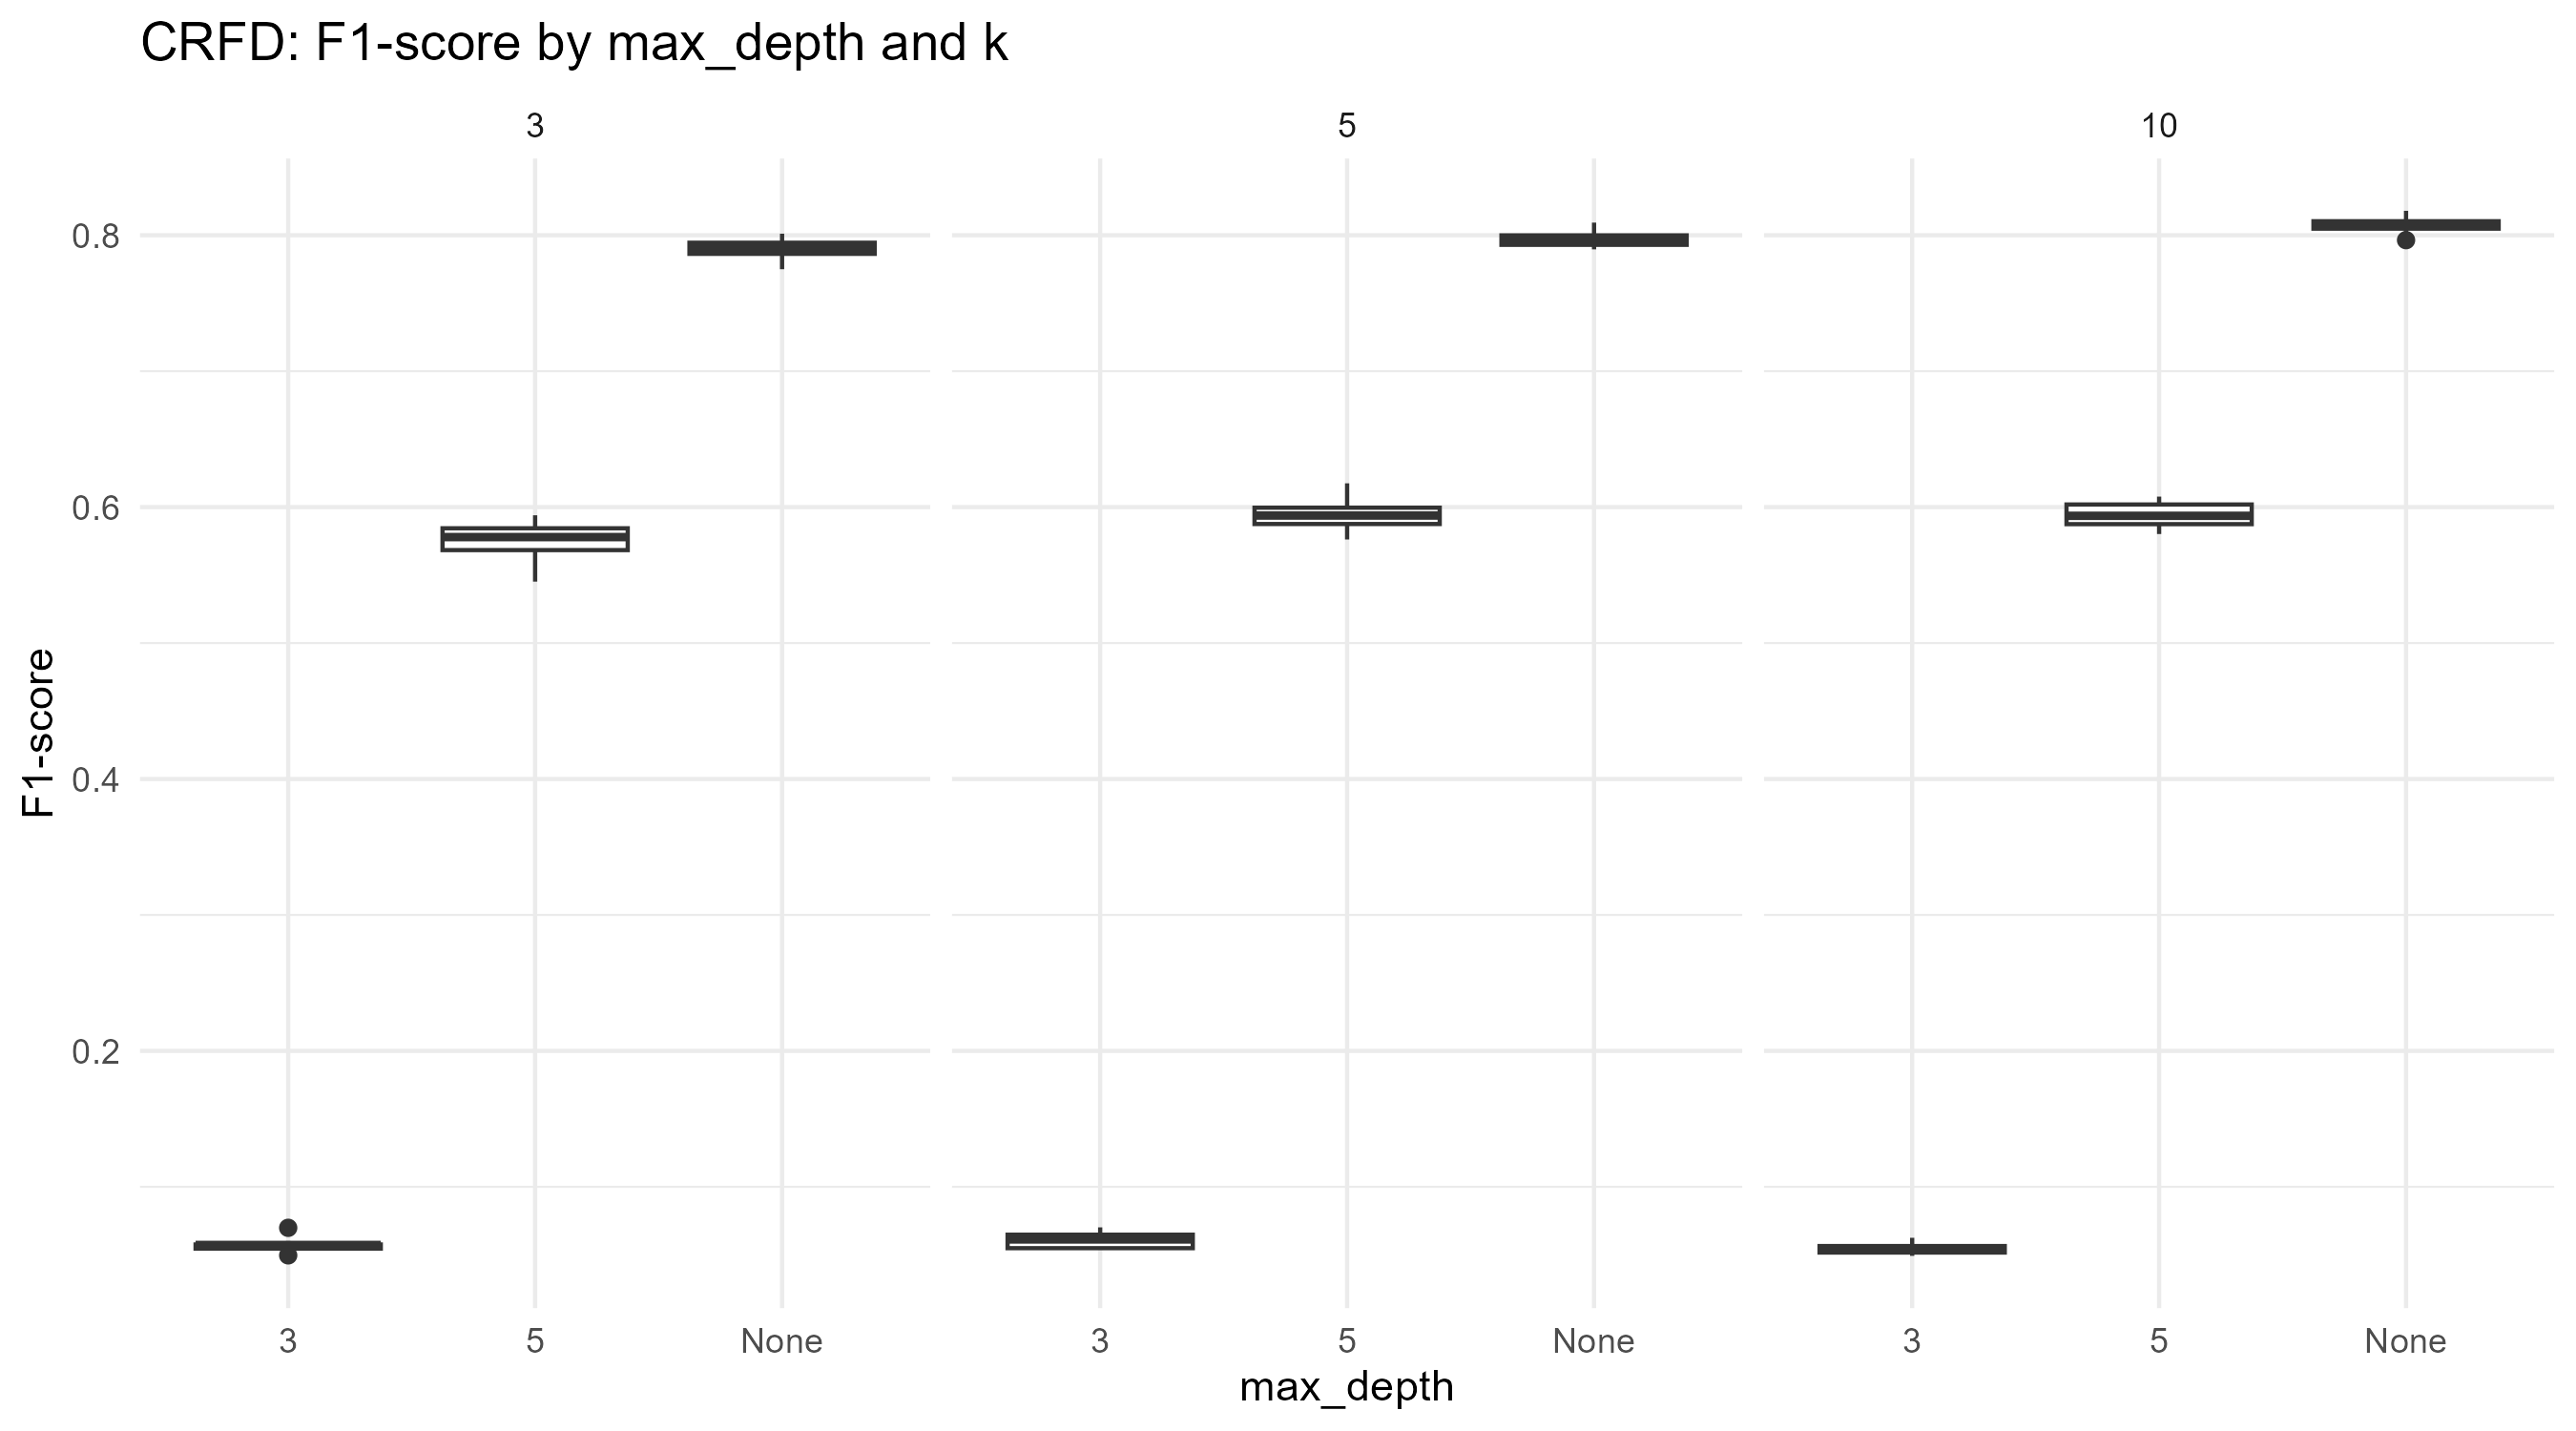
\includegraphics[width=0.92\textwidth]{outputs/r_crfd_boxplot.png}
    \caption{Boxplot F1-score theo \texttt{max\_depth}, phân tách theo từng mức $k$.}
    \label{fig:crfd_boxplot}
\end{figure}

Boxplot cho thấy sự khác biệt giữa các mức \texttt{max\_depth} là rất lớn. Với \texttt{max\_depth = 3}, F1 gần bằng 0.06, thấp hơn rất nhiều so với hai mức còn lại. Điều này cho thấy cây quá nông không đủ khả năng biểu diễn quan hệ giữa các biến đầu vào và trạng thái rời mạng. Khi tăng \texttt{max\_depth} lên 5, mô hình cải thiện đáng kể. Khi không giới hạn độ sâu, mô hình đạt hiệu năng cao nhất.

\subsection{Kiểm định Levene và Shapiro-Wilk}

Kiểm định Levene cho các tổ hợp nghiệm thức trong CRFD cho kết quả:
\[
F = 3.3086, \qquad p = 0.00255.
\]
Vì $p < 0.05$, có bằng chứng cho thấy phương sai giữa một số tổ hợp nghiệm thức không đồng nhất. Đây là điểm cần lưu ý khi diễn giải ANOVA. Tuy nhiên, do thiết kế cân bằng với 10 quan sát cho mỗi tổ hợp, kết quả ANOVA vẫn được dùng làm phân tích chính, đồng thời kết luận được hỗ trợ bằng bảng trung bình, khoảng tin cậy và đồ thị tương tác.

Kiểm định Shapiro-Wilk cho phần dư của mô hình CRFD cho kết quả:
\[
W = 0.97613, \qquad p = 0.09623.
\]
Vì $p > 0.05$, không có bằng chứng mạnh cho thấy phần dư lệch khỏi phân phối chuẩn.

\begin{figure}[H]
    \centering
    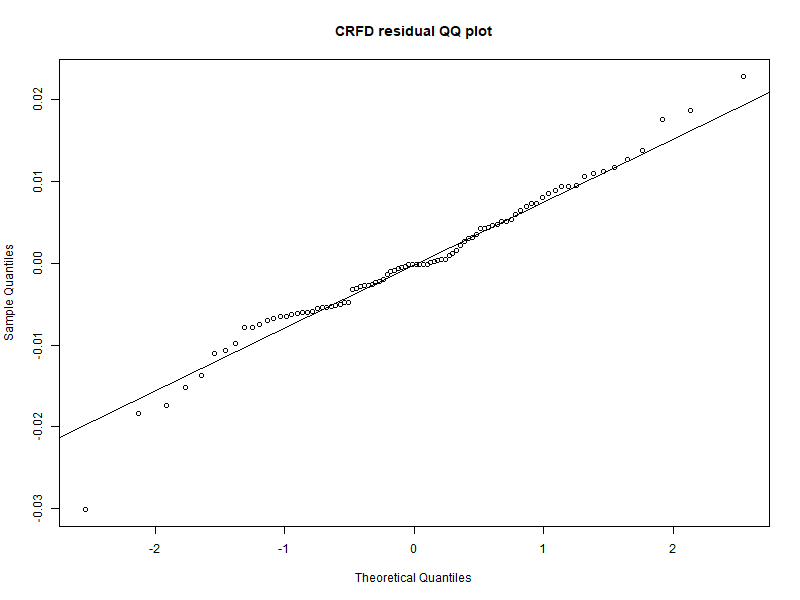
\includegraphics[width=0.72\textwidth]{outputs/r_crfd_qqplot.png}
    \caption{QQ plot phần dư của mô hình CRFD.}
    \label{fig:crfd_qqplot}
\end{figure}

\subsection{So sánh hậu nghiệm trong CRFD}

TukeyHSD cho yếu tố $k$ trong CRFD cho thấy:
\begin{itemize}
    \item $k=5$ cao hơn $k=3$ với chênh lệch 0.01015, $p = 0.0000591$.
    \item $k=10$ cao hơn $k=3$ với chênh lệch 0.01110, $p = 0.0000117$.
    \item $k=10$ không khác có ý nghĩa thống kê so với $k=5$, với $p = 0.9067$.
\end{itemize}

TukeyHSD cho yếu tố \texttt{max\_depth} cho thấy cả ba mức đều khác nhau có ý nghĩa thống kê. Chênh lệch giữa \texttt{max\_depth = 5} và \texttt{max\_depth = 3} là khoảng 0.5305, giữa \texttt{None} và 3 là khoảng 0.7409, và giữa \texttt{None} và 5 là khoảng 0.2104. Điều này tiếp tục khẳng định \texttt{max\_depth} là yếu tố có ảnh hưởng rất lớn đến hiệu năng mô hình.

\begin{figure}[H]
    \centering
    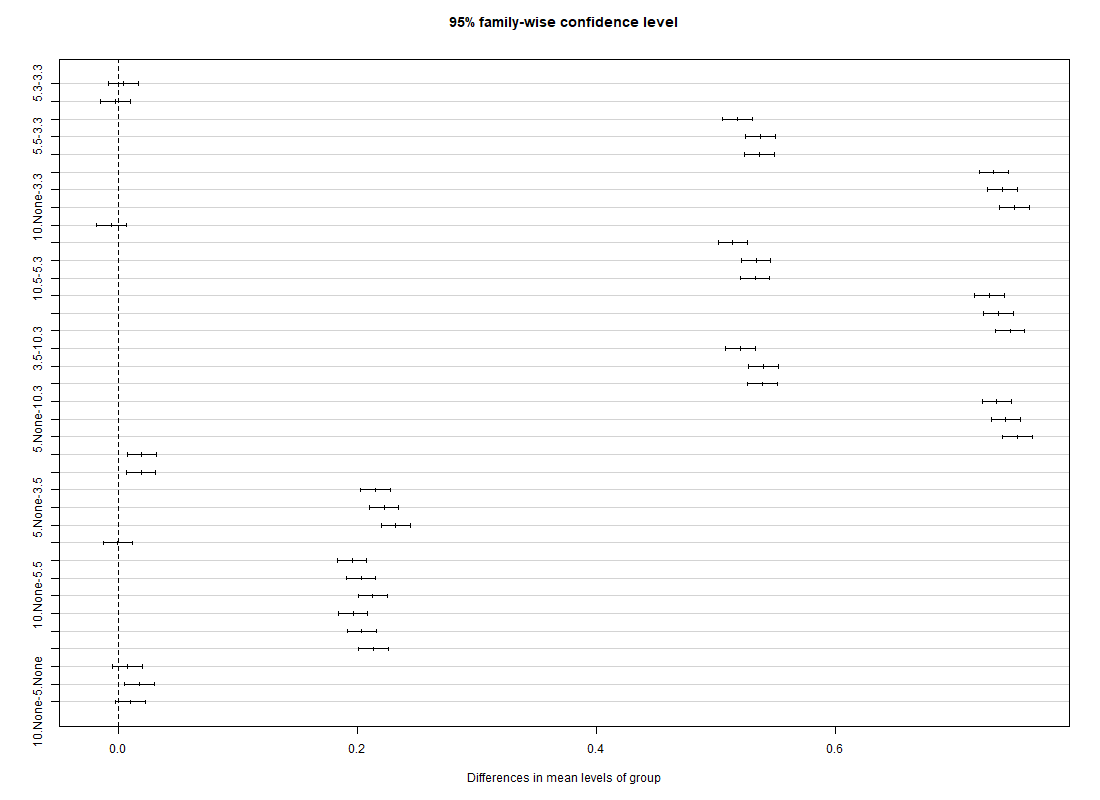
\includegraphics[width=0.88\textwidth]{outputs/r_crfd_tukey_group_plot.png}
    \caption{Đồ thị TukeyHSD cho các tổ hợp nghiệm thức trong CRFD.}
    \label{fig:crfd_tukey_group}
\end{figure}

% ============================================================
\section{Thảo luận}
% ============================================================

Kết quả từ hai thí nghiệm cho thấy số fold $k$ và siêu tham số \texttt{max\_depth} đều ảnh hưởng đến F1-score của mô hình Random Forest.

Trong thí nghiệm CRD, khi \texttt{max\_depth} không bị giới hạn, F1-score tăng dần từ $k=3$ đến $k=10$. Kết quả ANOVA và TukeyHSD đều cho thấy sự khác biệt giữa các mức $k$ là có ý nghĩa thống kê. Điều này cho thấy, trong bối cảnh thí nghiệm này, sử dụng nhiều fold hơn giúp đánh giá và huấn luyện mô hình ổn định hơn.

Trong thí nghiệm CRFD, yếu tố \texttt{max\_depth} có ảnh hưởng mạnh hơn nhiều so với $k$. Khi \texttt{max\_depth = 3}, mô hình cho F1 rất thấp, chứng tỏ cây quá nông dẫn đến underfitting. Khi \texttt{max\_depth = 5}, hiệu năng tăng đáng kể nhưng vẫn thấp hơn nhiều so với trường hợp không giới hạn độ sâu. Khi \texttt{max\_depth = None}, mô hình đạt F1 cao nhất.

Tương tác giữa $k$ và \texttt{max\_depth} có ý nghĩa thống kê. Điều này cho thấy ảnh hưởng của $k$ không giống nhau ở mọi mức \texttt{max\_depth}. Khi cây quá nông, thay đổi $k$ gần như không cải thiện hiệu năng đáng kể. Khi cây đủ sâu, đặc biệt là \texttt{max\_depth = None}, việc tăng $k$ từ 3 lên 10 làm F1 tăng rõ hơn.

Một điểm cần lưu ý là kiểm định Levene trong CRFD cho thấy phương sai giữa các tổ hợp nghiệm thức không hoàn toàn đồng nhất. Nguyên nhân có thể do các mức \texttt{max\_depth} tạo ra các vùng hiệu năng rất khác nhau, đặc biệt \texttt{max\_depth = 3} có F1 rất thấp và dao động nhỏ. Tuy nhiên, thiết kế thí nghiệm là cân bằng, mỗi tổ hợp có 10 quan sát, nên ANOVA vẫn có thể được sử dụng như phân tích chính, kết hợp với bảng trung bình và khoảng tin cậy để diễn giải kết quả.

% ============================================================
\section{Kết luận}
% ============================================================

Bài báo cáo đã xây dựng mô hình Random Forest để dự đoán khách hàng rời mạng trên bộ dữ liệu \texttt{mlc\_churn}. Các biến dư thừa về cước phí được loại bỏ dựa trên tương quan và ý nghĩa thực tiễn; biến \texttt{state} cũng được loại bỏ để giảm độ phức tạp của mô hình.

Kết quả thí nghiệm CRD cho thấy số fold $k$ có ảnh hưởng có ý nghĩa thống kê đến F1-score. Trong ba mức được xét, $k=10$ cho hiệu năng tốt nhất với F1 trung bình khoảng 0.807 và khoảng tin cậy 95\% là [0.803, 0.812].

Kết quả thí nghiệm CRFD cho thấy cả hai yếu tố $k$ và \texttt{max\_depth} đều có ảnh hưởng có ý nghĩa thống kê đến F1-score. Trong đó, \texttt{max\_depth} là yếu tố ảnh hưởng mạnh nhất. Trường hợp \texttt{max\_depth = None} cho hiệu năng cao nhất ở tất cả các mức $k$. Tổ hợp tốt nhất trong thí nghiệm là:
\[
k = 10, \qquad \texttt{max\_depth} = \texttt{None},
\]
với F1 trung bình khoảng 0.807.

Ngoài ra, tương tác giữa $k$ và \texttt{max\_depth} cũng có ý nghĩa thống kê, cho thấy tác động của số fold phụ thuộc vào độ sâu tối đa của cây. Nhìn chung, để đạt hiệu năng tốt cho bài toán này, nên sử dụng Random Forest không giới hạn độ sâu và đánh giá bằng repeated stratified k-fold với $k=10$.

% ============================================================
\section*{Tài liệu tham khảo}
\addcontentsline{toc}{section}{Tài liệu tham khảo}
% ============================================================

\begin{enumerate}
    \item Kuhn, M. \textit{modeldata: Data Sets Useful for Modeling Examples}. R package version 1.5.1, 2025.
    \item R Core Team. \textit{R: A Language and Environment for Statistical Computing}. R Foundation for Statistical Computing, Vienna, Austria, 2024.
    \item Breiman, L. Random Forests. \textit{Machine Learning}, 45, 5--32, 2001.
    \item Lawson, J. \textit{Design and Analysis of Experiments with R}. CRC Press, 2015.
\end{enumerate}

% ============================================================
\appendix
\section{Phụ lục: các file kết quả}
% ============================================================

Các file chính được tạo ra trong quá trình thực nghiệm gồm:
\begin{itemize}
    \item \texttt{outputs/crd\_results.csv}
    \item \texttt{outputs/crfd\_results.csv}
    \item \texttt{outputs/statistical\_analysis\_outputs.txt}
    \item \texttt{outputs/r\_crd\_summary\_mean\_ci.csv}
    \item \texttt{outputs/r\_crfd\_summary\_mean\_ci.csv}
    \item \texttt{outputs/r\_crd\_mean\_ci\_plot.png}
    \item \texttt{outputs/r\_crd\_boxplot.png}
    \item \texttt{outputs/r\_crd\_tukey\_plot.png}
    \item \texttt{outputs/r\_crfd\_interaction\_plot.png}
    \item \texttt{outputs/r\_crfd\_boxplot.png}
    \item \texttt{outputs/r\_crd\_qqplot.png}
    \item \texttt{outputs/r\_crfd\_qqplot.png}
\end{itemize}

\end{document}
